% !Mode:: "TeX:UTF-8"
\documentclass{article}
\usepackage{CJK}
\usepackage{graphicx}
\usepackage{subfigure}
%\usepackage{subfig}

\usepackage{makecell}
%\usepackage{cleveref}
%\Crefname{table}{Table}{Table}
%\Crefname{figure}{Fig.}{Fig.}

\usepackage{caption}
\usepackage{subcaption}


\begin{document}
\begin{CJK}{UTF8}{gbsn}
	

	
\section{exp}
\subsection{exp}

两张图并排,其中一张图还有两个子图
和floatrow这个包冲突,会报错:Package floatrow Error: Caption(s) lost. \\caption Flower two.之类的
这个方法就是Fig.\ref{fig:my_flower1}图片的label取不到
\begin{figure*}[!h]
	\setlength{\abovecaptionskip}{0pt}
	\setlength{\belowcaptionskip}{0pt}
	\centering
	\begin{minipage}[b]{0.4\textwidth}
		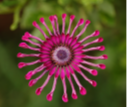
\includegraphics[width=\textwidth]{imgs/flower1.png}
		\caption{Flower one.}
		\label{fig:my_flower1}  %label必须放在caption的下面才行,否则引用的图片会是section的编号
	\end{minipage}
	\hfill % 这行如果去掉了,两张图片中间的空间就没有了
	\begin{minipage}[b]{0.55\textwidth}
		\subfigure[SL=0.5]{
			\label{fig:my_flower2_1} %% label for first subfigure
			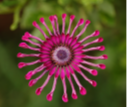
\includegraphics[width=0.31\textwidth]{imgs/flower1.png}
		}
		\subfigure[SL=0.5]{
			\label{fig:my_flower2_2} %% label for first subfigure
			
\includegraphics[width=0.31\textwidth]{imgs/flower2.png}
		}
		\caption{Flower two.}
	\end{minipage}
\end{figure*}



法二:子图模式,用subfig包
\iffalse    subfig和subfigure包有冲突,不能共用
\begin{figure*}[!h]
	\centering
	\subfloat[label 1]{{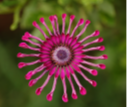
\includegraphics[width=5cm]{imgs/flower1.png} }}%
	\qquad
	\subfloat[label 2]{{
\includegraphics[width=5cm]{imgs/flower2.png} }}%
	\caption{2 Figures side by side}%
	\label{fig:example}%
\end{figure*}
\fi


法三:用subfigure包
%\iffalse    subfig和subfigure包有冲突,不能共用
\begin{figure*}[!h]
	\hfill
	\subfigure[Title A]{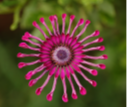
\includegraphics[width=5cm]{imgs/flower1.png}}
	\hfill
	\subfigure[Title B]{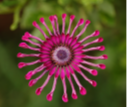
\includegraphics[width=5cm]{imgs/flower1.png}}
	\hfill
	\caption{Title for both}
\end{figure*}
%\fi

%法四:用minipage + subcaption(subcaption与subfigure冲突)
%\begin{figure*}[!h]
%	\setlength{\abovecaptionskip}{0pt}
%	\setlength{\belowcaptionskip}{0pt}
%	\centering
%	\begin{minipage}[b]{0.4\textwidth}
%		\centering
%		\subcaption{Beijing} {
%			\label{fig:map_gridding_bj} 
%			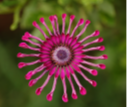
\includegraphics[width=0.9\textwidth]{imgs/flower1.png}
%		}
%	\end{minipage}
%	%\hfill
%	\begin{minipage}[b]{0.4\textwidth}
%		\centering
%		\subcaption{New York City} {
%			\label{fig:map_gridding_bj} 
%			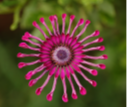
\includegraphics[width=0.9\textwidth]{imgs/flower1.png}
%		}
%	\end{minipage}
%	\caption{Map gridding of Beijing and New York City. The blue points denote the existing charging stations.}
%	The decimal degree of side length of grids in Beijing and New York is 0.02 and 0.01, respectively.
%	\label{fig:map_gridding}
%\end{figure*}



图片和表格并排, 用caption包, 参考:https://www.zhihu.com/question/29803796

\begin{figure*}[!h] 
	\begin{minipage}[b]{0.5\textwidth} 
		\centering 
		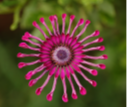
\includegraphics[width=0.8\textwidth]{imgs/flower1.png} 
		\caption{This is a Figure by a Table} 
		\label{fig:by:table} 
	\end{minipage}% 
	\begin{minipage}[b]{0.5\textwidth} 
		\centering
		\begin{tabular}{|c|c|} \hline 
			Day & Data \\ \hline\hline 
			Monday    & 14.6 \\ 
			Tuesday   & 14.3 \\ 
			Wednesday & 14.2 \\ 
			Thursday  & 14.5 \\ 
			Friday    & 14.9 \\ \hline 
		\end{tabular} 
		\captionof{table}{This is a table}
		\label{table:by:fig} 
	\end{minipage} 
\end{figure*}


2*2布局的图片

\begin{figure*}[!h] 
	\centering 
	\subfigure[subfigure 1-1]{\label{fig:subfig:a}
		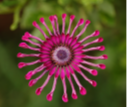
\includegraphics[width=0.45\linewidth]{imgs/flower1.png}}
	\hspace{0.01\linewidth}
	\subfigure[subfigure 1-2]{\label{fig:subfig:b}
		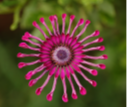
\includegraphics[width=0.45\linewidth]{imgs/flower1.png}}
	\vfill
	\subfigure[subfigure 2-1]{\label{fig:subfig:a}
		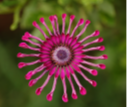
\includegraphics[width=0.45\linewidth]{imgs/flower1.png}}
	\hspace{0.01\linewidth}
	\subfigure[subfigure 2-2]{\label{fig:subfig:b}
		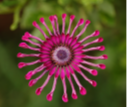
\includegraphics[width=0.45\linewidth]{imgs/flower1.png}}
	\caption{two figures}
	\label{fig:subfig}
\end{figure*}


让两个并列但大小不等的图,垂直居中:http://www.ctex.org/documents/latex/graphics/node109.html
\begin{figure*}[!h] 
	\centering 
	\begin{minipage}[c]{0.5\textwidth} 
		\centering 
		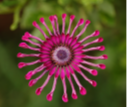
\includegraphics[width=1in]{imgs/flower1.png} 
	\end{minipage}% 
	\begin{minipage}[c]{0.5\textwidth} 
		\centering 
		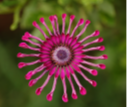
\includegraphics[width=2in]{imgs/flower1.png} 
	\end{minipage} 
	\caption{Centers Aligned Vertically} 
\end{figure*}




\begin{figure*}[!h] 
	\centering 
	\begin{minipage}[c]{0.3\textwidth} 
		\centering 
		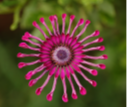
\includegraphics[width=\textwidth]{imgs/flower1.png}
		\caption{Result of DECO.}
		%\label{fig:sdbscan_cluster}  
	\end{minipage}% 
	\begin{minipage}[c]{0.5\textwidth} 
		\centering 
		\subfigure[1st Round]{
			%\label{fig:dbscan1}
			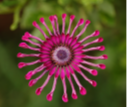
\includegraphics[width=0.45\linewidth]{imgs/flower1.png}}
		\hspace{0.01\linewidth}
		\subfigure[2nd Round]{
			%\label{fig:dbscan2}
			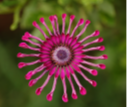
\includegraphics[width=0.45\linewidth]{imgs/flower1.png}}
		\vfill
		\subfigure[3rd Round]{
			%\label{fig:dbscan3}
			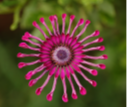
\includegraphics[width=0.45\linewidth]{imgs/flower1.png}}
		\hspace{0.01\linewidth}
		\subfigure[Integration]{
			%\label{fig:dbscanmerge}
			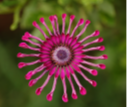
\includegraphics[width=0.45\linewidth]{imgs/flower1.png}}
		
		\caption{Multiple Rounds DBSCAN}
		\label{fig:subfig}
	\end{minipage} 
\end{figure*}




\end{CJK}
\end{document}